\documentclass[10pt,a4paper]{article}
\usepackage[margin=1.8cm]{geometry}
\usepackage[T1]{fontenc}
\input{glyphtounicode}\pdfgentounicode=1
\pdfinterwordspaceon
\usepackage{lmodern,microtype,graphicx,booktabs,longtable,tabularx,array,enumitem,amsmath,amssymb,makecell,multirow,upquote}
\usepackage[table]{xcolor}
\usepackage{fvextra}
\usepackage[most]{tcolorbox}
\usepackage[font=small,labelfont=bf]{caption}
\usepackage[colorlinks=true,linkcolor=blue!50!black,urlcolor=blue!50!black]{hyperref}
\setlist{nosep,leftmargin=1.3em}
\setlength{\parindent}{0pt}\setlength{\parskip}{4pt}
\pagestyle{empty}% no page numbers: copying across a page break stays clean

\newtcolorbox{rev}[1][Reviewer]{breakable,enhanced,colback=gray!7,colframe=gray!55,title={#1},fonttitle=\bfseries\small,fontupper=\small\itshape,left=4pt,right=4pt,top=2pt,bottom=2pt}
\newtcolorbox{todo}[1][What to do]{breakable,enhanced,colback=blue!3,colframe=blue!45!black,title={#1},fonttitle=\bfseries\small,fontupper=\small,left=4pt,right=4pt,top=2pt,bottom=2pt}
\newtcolorbox{priv}[1][For you only (not for the reviewer)]{breakable,enhanced,colback=red!3,colframe=red!55!black,title={#1},fonttitle=\bfseries\small,fontupper=\small,left=4pt,right=4pt,top=2pt,bottom=2pt}
\newtcolorbox{codebox}[1]{breakable,enhanced,colback=yellow!4,colframe=orange!60!black,title={#1},fonttitle=\small,left=3pt,right=3pt,top=1pt,bottom=1pt,boxrule=0.6pt}
\newtcolorbox{respbox}[1]{breakable,enhanced,colback=green!3,colframe=green!35!black,title={#1},fonttitle=\bfseries\small,left=3pt,right=3pt,top=1pt,bottom=1pt}
\newtcolorbox{prevbox}{breakable,enhanced,colback=white,colframe=gray!40,title={Preview (how it compiles)},fonttitle=\small,left=2pt,right=2pt,top=1pt,bottom=1pt,boxrule=0.4pt}

\fvset{breaklines=true,breaksymbolleft={},breaksymbolright={},breakindent=0pt,fontsize=\footnotesize}
\newcommand{\snip}[1]{\begin{codebox}{LaTeX to paste \textbullet\ \texttt{snippets/\detokenize{#1}.tex}}\VerbatimInput{../snippets/#1.tex}\end{codebox}}
\newcommand{\resp}[1]{\begin{respbox}{Response letter text (LaTeX) \textbullet\ \texttt{snippets/resp\_\detokenize{#1}.tex}}\VerbatimInput{../snippets/resp_#1.tex}\end{respbox}}
\newcommand{\preview}[1]{\begin{prevbox}\begingroup\footnotesize\setlength{\tabcolsep}{2.5pt}%
\renewenvironment{table}[1][]{\centering}{}\renewenvironment{table*}[1][]{\centering}{}%
\renewcommand{\caption}[1]{\par{\itshape ##1}\par\smallskip}\renewcommand{\label}[1]{}\renewcommand{\cite}[1]{[ref]}%
\input{../snippets/#1.tex}\endgroup\end{prevbox}}
\newcounter{stepc}
\newcommand{\step}[1]{\par\medskip\noindent\refstepcounter{stepc}{\color{blue!45!black}\textbf{Step \arabic{stepc}}}\quad\textbf{#1}\par}
\newcommand{\find}[1]{\par\noindent{\small\textbf{Find:}~\textsf{``#1''}}\par}
\newcommand{\FILL}[1]{\textcolor{orange!85!black}{\textbf{[FILL: #1]}}}
\newcommand{\fig}[2][\linewidth]{\begin{center}\includegraphics[width=#1]{#2}\end{center}}
\newcommand{\st}[1]{Step~\ref{#1}}

\begin{document}
\begin{center}
{\LARGE\bfseries Manuscript AIS 3400076: revision workbook}\\[4pt]
{\large Every editor and reviewer comment, exact edits in LaTeX, and the response letter}\\[4pt]
{\small Built from the decision letter (22 Sep 2026), the submitted manuscript and SI, the repository code and the original datasets.}
\end{center}

\section*{How to use this document}
\begin{enumerate}
\item Work through the numbered \textbf{Steps}. Each gives \emph{where} (manuscript or SI, section, paragraph), the current text to \textbf{find} as printed in the submitted PDF, and the LaTeX to paste in a yellow box.
\item Select the text in a yellow box and copy it (the pages have no numbers, so a box that continues on the next page also copies cleanly). Every box is also a file in \texttt{snippets/} with the name shown in its title; copying from the file is the safest option.
\item Green boxes are the response-letter text for each comment. They are already assembled, with the reviewer quotes, in \texttt{snippets/response\_letter.tex}, which compiles as is; \texttt{AIS\_3400076\_response\_letter.pdf} is the compiled version.
\item Grey boxes quote the reviewer, blue boxes say what to do, and red boxes are notes for you only. \FILL{...} marks information only you have; search the snippets for \texttt{[FILL} and \texttt{[CONFIRM]} before submission.
\item Mark the changes in the revised manuscript (the editor may ask for it), e.g.\ by wrapping each pasted text in \verb|\textcolor{blue}{...}|.
\end{enumerate}

\textbf{Symbols in the snippets.} The PDF does not expose your macros, so the snippets use plain notation: $\mathbf{l}$ tendon lengths, $\bar{\mathbf{l}}$ their mean, $\mathbf{l}_{\mathrm{enc}}$ encoder reading, $\mathbf{p}$ tip pose, $\mathbf{t}$ tip position, $\mathbf{J}$ Jacobian, $f_p^n$, $f_C^n$, $N_l^1$, $N_p^3$, $N_l^3$, $N_C$ networks, $W^3$ planner, $\zeta$ weight of the secondary term, $H(\mathbf{l})$ secondary cost, $\boldsymbol{\xi}$ and $\mathbf{q}$ PCC parameterizations. Replace them with your own macros where they differ.

\textbf{Numbering of new SI items.} So that the existing SI numbers (Tables~S1--S6, Figs.~S1--S6) stay unchanged, put \emph{all new table and figure environments at the end of the SI} (\st{st:siend}), in this order: Tables~S7 (path errors), S8 and S9 (targets), S10 (comparison), S11 (reproducibility), S12 (dataset composition), S13 (ablation), S14 (train/test overlap); then Figs.~S7 (error vs.\ bending), S8 (ablation), S9 (coverage). The text snippets refer to these numbers. New SI text goes into the sections named in each step, including two new subsections (5.3 and 6.6).

\textbf{What was verified.} Table~1, Table~S6, Fig.~5c, Fig.~8b, Table~2 and the bars of Fig.~7 were reproduced from the repository and the original datasets with the original split. Every notebook seeds Python, NumPy and PyTorch with 42 before splitting. Table~S5 is reproduced within 0.02~mm and $0.08^\circ$.

\textbf{Graphs.} Every new or revised graph comes from a notebook in the repository, with its executed output, so you can take it from there:
\begin{itemize}
\item \texttt{SINGLE/SINGLE\_revision\_figures.ipynb}: Fig.~5b with equal axes (\texttt{fig5b\_equal\_axes.pdf}) and Fig.~S4 with target IDs (\texttt{figS4\_matched\_ids.pdf}).
\item \texttt{MULTI/MULTI\_revision\_figures.ipynb}: Fig.~7 per point (\texttt{fig7\_per\_point.pdf}), Fig.~S7 error vs.\ bending (\texttt{bending\_error.pdf}), Figs.~S5 and S6 with target IDs (\texttt{figS5\_matched\_ids.pdf}, \texttt{figS6\_matched\_ids.pdf}), Fig.~S8b data-driven ablation (\texttt{ik\_ablation.pdf}), and the Fig.~3 and Fig.~4c diagrams (\texttt{fig3\_network\_map.pdf}, \texttt{fig4c\_signal\_flow.pdf}). Run the SINGLE notebook first.
\item Already in the repository: Fig.~S8a (\texttt{MULTI\_nullspace\_ablation.ipynb}, \texttt{nullspace\_ablation.pdf}) and Fig.~S9 (\texttt{SINGLE\_workspace\_coverage.ipynb} and \texttt{MULTI\_workspace\_coverage.ipynb}).
\end{itemize}
Each notebook saves its PDFs in the \texttt{results/} folder of its arm.

\textbf{Files} (in \texttt{REVIEW\_TO\_DELETE/} of the repository): this guide, \texttt{AIS\_3400076\_response\_letter.pdf}, the original review PDFs, and \texttt{AIS\_3400076\_revision/} with the sources:
\begin{itemize}
\item \texttt{snippets/}: every LaTeX box, and \texttt{response\_letter.tex}.
\item \texttt{build/main.tex} and \texttt{crops/}: source of this guide.
\item \texttt{scripts/} and \texttt{data/}: the analyses behind the numbers and tables; \texttt{scripts/snippets.py} regenerates the snippets.
\end{itemize}

\subsection*{Checklist: every comment and where it is handled}
\small
\begin{longtable}{p{1.0cm}p{5.6cm}p{8.4cm}p{1.2cm}}
\toprule
ID & Comment & What changes & Section\\\midrule\endhead
G1--G6 & Editor: title, references, acronyms, figure text, copyright, DOIs & Acronym pass, captions, DOIs, statement & \ref{sec:editor}\\\midrule
1 & Role of visual sensing in control & Abstract, contributions, Sec.~3.3, Alg.~1, Fig.~4c, Conclusion & \ref{sec:f4}, \ref{sec:ctrl}\\
2 & Originality vs.\ prior work & Intro paragraph, contributions, Table~S10, 4 references & \ref{sec:comp}\\
3 & Scalability claim & Sec.~3.1, Intro, contributions, Conclusion & \ref{sec:claims}\\
4 & Ground truth of the reconstruction & Assumptions (Sec.~2.2), Sec.~4.2.2, SI 4.2, Fig.~S2 & \ref{sec:data}, \ref{sec:fs2}\\
5 & Arc-length inconsistency & Eqs.~4--6, SI 2.2, SI Eqs.~S3--S4, Table~S1 & \ref{sec:model}\\
6 & Secondary objective & Sec.~3.3.2 wording, SI 5.3, Table~S13, Fig.~S8 & \ref{sec:results}\\
7 & Coverage of the control evaluation & Sec.~3.2 range, Secs.~4.1.4, 4.2.6, SI 6.3, Tables~S8--S9, Fig.~S9, Sec.~5 & \ref{sec:results}\\
8 & Train/test independence & Secs.~3.1.1, 3.2, SI 4.1, Tables~S12, S14 & \ref{sec:data}\\
9 & Reproducibility & Table~S11, SI 3.1, Sec.~5 (lighting) & \ref{sec:nets}, \ref{sec:hw}\\
10 & Figures 1B, 2, 3, 5 & Part~1 & \ref{sec:figs}\\\midrule
11 & ``Markerless'' & Contribution 1 & \ref{sec:claims}\\
12 & Section vs.\ segment & Replacement list & \ref{sec:claims}\\
13 & Number of tendons, preload & Sec.~2.1 & \ref{sec:hw}\\
14 & Camera details & Sec.~2.1, Table~S11 & \ref{sec:hw}\\
15 & ``Simultaneous'' acquisition & Sec.~2.1, Fig.~1 caption & \ref{sec:hw}, \ref{sec:f1}\\
16 & Sine/cosine, loss balance & SI 3.1 & \ref{sec:nets}\\
17 & Sign in Eq.~S11, highlighted pixels & SI 3.2, Fig.~4 caption & \ref{sec:nets}, \ref{sec:f4}\\
18 & PCC line in Alg.~1 & Alg.~1, Sec.~3.3.2 & \ref{sec:ctrl}\\
19 & Jacobian notation & Secs.~3.3, 3.3.1, Eq.~7, Algs.~1--2, Fig.~S3, Table~S2 & \ref{sec:ctrl}\\
20 & Open-loop baselines, terminology & Sec.~3.3.1, ``feedforward'' & \ref{sec:ctrl}\\
21 & Percentage denominators & Secs.~4.1.1, 4.1.4, 4.2.1, 4.2.3, 4.2.4, 4.2.6 & \ref{sec:results}\\
22 & Fig.~5b scaling & Fig.~5b, caption & \ref{sec:f5}\\
23 & Fig.~7 statistic & Fig.~7, caption, Secs.~4.1.2, 4.2.2 & \ref{sec:f7}\\
24 & Table~1 robust statistics & Table~1, Sec.~4.2.1 & \ref{sec:results}\\
25 & Bending claim & Fig.~S7, Secs.~4.1.1, 4.2.1 & \ref{sec:results}\\
26 & Figs.~6, 9, 10 details, path errors & Captions, Table~S7 & \ref{sec:f6}\\
27 & Demonstrated vs.\ proposed & Sec.~5 & \ref{sec:claims}\\\midrule
28 & Fig.~S2b numbers & Fig.~S2 caption, SI 4.2 & \ref{sec:fs2}\\
29 & Table~S6 skew & Table~S6, SI 6.1 & \ref{sec:results}\\
30 & Figs.~S4--S6 IDs, colors & Figures, captions & \ref{sec:fs456}\\
31 & Tables~S3/S4 composition & SI 4.1, Table~S12 & \ref{sec:data}\\
\bottomrule
\end{longtable}
\normalsize

%==========================================================================
\clearpage
\section{Figures and captions}\label{sec:figs}
\begin{rev}[Reviewer, Comment 10]
Several figures---particularly Figs.~1B, 2, 3, and 5---are difficult to interpret. [\dots] In particular, Figure~3 requires attention. [\dots] The paper should use a consistent flow direction, label all network inputs and outputs, and distinguish clearly between the networks used for pose estimation, curvature reconstruction, forward kinematics, and inverse kinematics.
\end{rev}

\textbf{Summary.} Graphics change only where a comment asks for it: Fig.~3 (redraw), Fig.~7 (new statistic) and Figs.~S4--S6 (target IDs, shared colors). Fig.~4c gets one added block and Fig.~5b equal axes. All other figures change only in their captions. Three new SI figures are added (S7--S9).

\small
\begin{tabularx}{\linewidth}{lXl}
\toprule
Figure & Change & Type\\\midrule
1 & Software synchronization, ``sections'', every label of panel b & caption\\
2 & $L_1$--$L_4$ vs.\ tendons & caption\\
3 & Network names, inputs/outputs, sizes, one flow direction & redraw + caption\\
4 & Grad-CAM definition (a); encoder path, curvature outside the loop (c) & small edit + caption\\
5 & Equal axis scaling in b; CL/OL and error bars in c & small edit + caption\\
6, 9, 10 & Start, direction, cycles, single run, ``open-loop''; path errors & caption + Table~S7\\
7 & Per-point error vs.\ normalized arc length & redraw + caption\\
8, S1 & ``section''; CL/OL; error bars & caption\\
S2 & Configurations, interval, independence & caption\\
S3 & Jacobian symbols & small edit\\
S4--S6 & Target IDs, shared color scales & redraw + caption\\
S7--S9 (new) & Error vs.\ bending; secondary-objective ablation; coverage & new\\
\bottomrule
\end{tabularx}
\normalsize

%--------------------------------------------------------------------------
\subsection{Figure 1}\label{sec:f1}
\fig[0.9\linewidth]{../crops/fig1_annot.png}
\begin{rev}[Reviewer, minor comments 12 and 15]
Use either `section' or `segment' consistently [\dots] The claim that images are acquired simultaneously should be supported by the synchronization method as this type software capture is not necessarily simultaneous hardware triggering.
\end{rev}
\step{Manuscript, Fig.~1: replace the whole caption.}\label{st:fig1}
The graphic stays as it is. The new caption:
\begin{itemize}
\item names every element of panel b;
\item expands the acronyms of panel a (BW, FE, FC);
\item describes the software synchronization (in the code, each camera is read in its own thread and the latest frame is used; there is no hardware trigger).
\end{itemize}
\snip{fig1_caption}
\begin{priv}
Check that $S_{\mathrm{I}}$--$S_{\mathrm{III}}$ in Fig.~1b are the section base frames; if they denote something else, change that half-sentence.
\end{priv}

\subsection{Figure 2}
\fig[0.55\linewidth]{../crops/fig2_annot.png}
\step{Manuscript, Fig.~2: replace the whole caption.}
Graphic unchanged. The confusing point is that four arcs $L_1$--$L_4$ are drawn next to three tendons; the caption now says what they are.
\snip{fig2_caption}

\subsection{Figure 3}
\fig[0.95\linewidth]{../crops/fig3_annot.png}
\step{Manuscript, Fig.~3: redraw (explicitly requested).}
Keep the two panels and their content, and change:
\begin{enumerate}
\item One flow direction, left to right, in both panels.
\item The network name on each output path: $f_p^1$, $f_C^1$ (single), $f_p^3$, $f_C^3$ (multi) in panel a; $N_l^1$ and $N_C$ on panel b.
\item Sizes: input $n \times 480 \times 640$; GAP output 1280; heads ``$1280 \to 6$'' and ``$1280 \to 5|4|3$'' ($n=1$), ``$1280 \to 512 \to 18$'' and ``$1280 \to 512 \to 15|12|9$'' ($n=3$). Marker \textcircled{\small 1}: the single box ``Linear Layer'' is wrong for $n=3$, whose heads have two layers.
\item One color per role: pose (green), curvature (orange), forward kinematics (yellow), inverse kinematics (purple).
\item Panel b (marker \textcircled{\small 2}) is the residual MLP of $N_l^1$ and $N_C$. Add a small box next to it: ``$N_p^3$: $9 \to 4\times128$ ELU $\to 6$; $N_l^3$: $6 \to 4\times128$ ELU $\to 9$, trained through the frozen $N_p^3$''.
\end{enumerate}
Template generated from the code (\texttt{MULTI/results/fig3\_network\_map.pdf}, from \texttt{MULTI\_revision\_figures.ipynb}):
\fig[0.95\linewidth]{../../../MULTI/results/fig3_network_map.pdf}
\step{Manuscript, Fig.~3: replace the whole caption.}
\snip{fig3_caption}

\subsection{Figure 4}\label{sec:f4}
\fig[0.95\linewidth]{../crops/fig4_annot.png}
\begin{rev}[Reviewer, Comment 1 (excerpt) and minor comment 17]
The abstract, contribution list, Fig.~4c, and conclusion should clearly distinguish: camera-based pose estimation used for control; encoder measurements used to calculate the Jacobian and null-space term; and image-based PPC reconstruction evaluated as a separate sensing capability. [\dots] clarify how the highlighted pixels are the regions used for prediction.
\end{rev}
\step{Manuscript, Fig.~4c: add one block and one arrow (marker \textcircled{\small 2}).}
Add a block ``Encoders'' that reads $\mathbf{l}$ (the output of the $1/s$ block). Draw an arrow from it to the box ``Model-based (PCC, Null-Space)'' and label it ``$\mathbf{l}$ (model-based only)''. Optionally, add a dashed block ``$f_C$ (curvature CNN): reconstruction output, not in the loop'', fed by ``Cameras''. Sketch:
\fig[0.95\linewidth]{../../../MULTI/results/fig4c_signal_flow.pdf}
(\texttt{MULTI/results/fig4c\_signal\_flow.pdf}, from \texttt{MULTI\_revision\_figures.ipynb}.)
\step{Manuscript, Fig.~4: replace the whole caption (covers 4a and 4c).}
\snip{fig4_caption}

\subsection{Figure 5}\label{sec:f5}
\fig[0.95\linewidth]{../crops/fig5_annot.png}
\begin{rev}[Reviewer, minor comment 22]
Figure~5b intentionally uses nonuniform axis scaling. This visually distorts the reconstructed shapes. Use equal spatial scaling where possible or add a second undistorted view and explicit scale bars.
\end{rev}
\step{Manuscript, Fig.~5b: equal axis scaling (marker \textcircled{\small 1}).}
In the plotting code of the two shape panels (GT and CNN), set \verb|ax.set_aspect('equal')| and give both panels the same limits (e.g.\ $x$ 0--60~mm, $z$ 0--150~mm). Equal axes make the panels narrow, so the simplest layout is one panel with GT (solid) and CNN (dashed) overlaid. The right panel below shows this layout, produced from the same models (\texttt{SINGLE/results/fig5b\_equal\_axes.pdf}, from \texttt{SINGLE\_revision\_figures.ipynb}):
\fig[0.7\linewidth]{../../../SINGLE/results/fig5b_equal_axes.pdf}
\step{Manuscript, Fig.~5: replace the whole caption.}\label{st:fig5}
\snip{fig5_caption}

\subsection{Figures 6, 9 and 10}\label{sec:f6}
\fig[0.85\linewidth]{../crops/fig6_annot.png}
\fig[0.85\linewidth]{../crops/fig9_annot.png}
\fig[0.7\linewidth]{../crops/fig10_annot.png}
\begin{rev}[Reviewer, minor comments 20 and 26]
`Open-loop' and `feedforward' should be used consistently. [\dots] For Figs.~6, 9, and 10, identify the start direction, waypoint order, number of completed cycles, and whether the plotted paths are one run or an average. Add quantitative path errors in the caption or an accompanying table.
\end{rev}
Facts from the logged trajectories:
\begin{itemize}
\item Every path starts at angle 0, i.e.\ at $(r, 0)$ relative to the circle center.
\item It visits the 30 vertices counter-clockwise (top view) and completes one cycle.
\item Each plotted path is a single run.
\end{itemize}
The panel titles already say ``open-loop''; only the captions say ``feedforward''.
\step{Manuscript, Figs.~6, 9 and 10: replace the three captions.}
\snip{fig6_caption}
\snip{fig9_caption}
\snip{fig10_caption}
\step{SI, end of the document: add Table~S7 (path errors, generated from the repository's \texttt{PathErrorMetrics} files).}
\snip{tab_S7_paths}
\preview{tab_S7_paths}

\subsection{Figure 7}\label{sec:f7}
\fig[0.5\linewidth]{../crops/fig7_annot.png}
\begin{rev}[Reviewer, minor comment 23]
Figure~7 alternates among `cumulative 3D error,' `sum of 3D errors,' and `average 3D error for each point.' Define the statistic exactly. Summing three points for the single-section arm and nine for the multi-section arm also prevents direct comparison. Per-point RMSE or error versus normalized arc length would be clearer.
\end{rev}
\step{Manuscript, Fig.~7: replace the graphic with the per-point version.}
The new version uses the same models and the same test set. The bar heights of the current figure (7.8, 7.9, 8.3~mm and 209, 203, 198~mm) are the sums of the per-point means shown here. Use \texttt{MULTI/results/fig7\_per\_point.pdf} (from \texttt{MULTI\_revision\_figures.ipynb}) as is, or replot it in your style (median and interquartile range against $s/L_{\mathrm{tot}}$):
\fig[0.9\linewidth]{../../../MULTI/results/fig7_per_point.pdf}
\step{Manuscript, Fig.~7: replace the whole caption.}\label{st:fig7}
\snip{fig7_caption}
\step{Manuscript, Section~4.1.2, last two sentences: replace.}
\find{Fig. 7a reports the average 3D error for each point, as well as the cumulative standard deviations across all curvature models. Although mean values are comparable, the standard deviation decreases with increasing model descriptiveness.}
\snip{text_412_fig7}
\step{Manuscript, Section~4.2.2, last sentence: replace.}
\find{Errors grow toward the distal tip; all models provide similar approximations, though increasing model complexity reduces variance.}
\snip{text_422_fig7}
\begin{priv}
Why the standard-deviation sentences go: recomputed on the test set, the spread does not decrease with model complexity. The standard deviation of the summed error is 6.55, 6.27 and 7.34~mm (constant, affine, quadratic) on the single section and 183, 188 and 171~mm on the multi-section arm. The new sentences only state what the per-point figure shows.
\end{priv}

\subsection{Figure 8}
\step{Manuscript, Fig.~8: replace the whole caption.}\label{st:fig8}
\snip{fig8_caption}

\subsection{Figure S1}
\step{SI, Fig.~S1: replace the whole caption (``multi-segment'', ``ends'').}\label{st:figS1}
\snip{figS1_caption}

\subsection{Figure S2}\label{sec:fs2}
\fig[0.55\linewidth]{../crops/figS2_annot.png}
\begin{rev}[Reviewer, Comment 4 (excerpt) and SI comment 28]
Fig.~S2b does not provide sufficient validation of N\_C: numerical errors, sample count, data split, and confidence intervals are missing. It is also unclear whether its validation configurations are independent of the data used to train N\_C and the three-section curvature estimator. [\dots] Fig.~S2b should report the numerical N\_C error for each curvature model, the number of validation configurations, and whether the bars show standard deviation, standard error, or another interval.
\end{rev}
What the code shows:
\begin{itemize}
\item There are 20 configurations (\texttt{MULTI\_curvature\_checks.py}), posed manually with all markers visible and recorded in a separate session.
\item Each bar is the sum over the nine points of the mean error per point.
\item The error bars are the sample standard deviation (ddof\,=\,1) of the per-configuration sum.
\item $N_C$ was trained on single-section data only.
\end{itemize}
\step{SI, Fig.~S2: replace the whole caption.}
\snip{figS2_caption}
The $N_C$ numbers go into SI Section~4.2 (\st{st:si42}).
\begin{priv}
Read note~\ref{priv:s2b} in Section~\ref{sec:private} before finalizing anything that cites values of Fig.~S2b.
\end{priv}

\subsection{Figure S3}
\fig[0.85\linewidth]{../crops/figS3_annot.png}
\step{SI, Fig.~S3: change the symbols in the blocks (marker \textcircled{\small 1}).}\label{st:figS3}
Model-based panel: the Jacobian block becomes $\mathbf{J}^{\#}$ of $\mathbf{J}_{l\to p}(\mathbf{l})$. Data-driven panel: $\hat{\mathbf{J}}_{p\to l}$. This is the notation of Section~\ref{sec:ctrl}. Caption unchanged.

\subsection{Figures S4--S6}\label{sec:fs456}
\begin{minipage}{0.48\linewidth}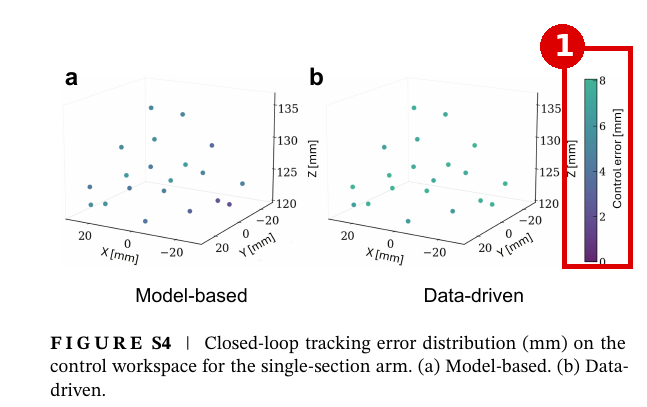
\includegraphics[width=\linewidth]{../crops/figS4_annot.png}\end{minipage}\hfill
\begin{minipage}{0.48\linewidth}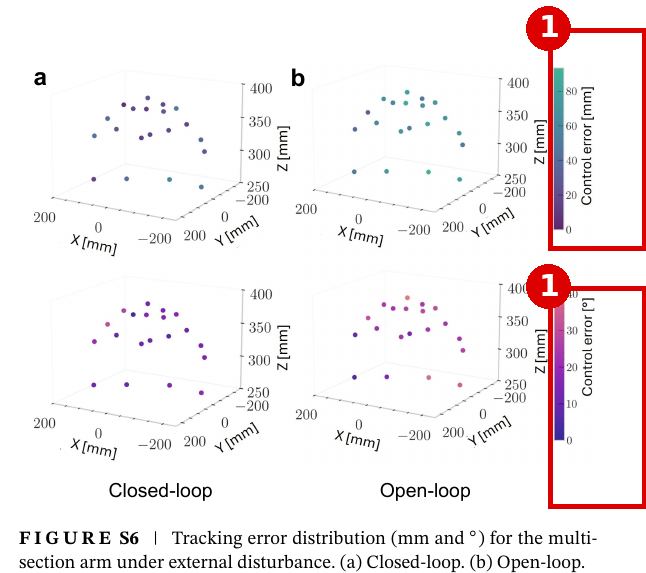
\includegraphics[width=\linewidth]{../crops/figS6_annot.png}\end{minipage}
\begin{rev}[Reviewer, SI comment 30]
Figs.~S4--S6 should use matched target identifiers or connecting pairs so the reader can compare the same workspace locations across controllers. Use consistent color limits when the goal is direct visual comparison.
\end{rev}
\step{SI, Figs.~S4--S6: replace the graphics.}
Same data and plots, with two changes:
\begin{itemize}
\item Each target carries its ID (1--20, the same as in Tables~S8 and S9).
\item Each figure uses one color scale per quantity; marker \textcircled{\small 1} shows the current independent color bars.
\end{itemize}
Ready to use: \texttt{SINGLE/results/figS4\_matched\_ids.pdf} (\texttt{SINGLE\_revision\_figures.ipynb}), \texttt{MULTI/results/figS5\_matched\_ids.pdf} and \texttt{figS6\_matched\_ids.pdf} (\texttt{MULTI\_revision\_figures.ipynb}).
\fig[0.7\linewidth]{../../../SINGLE/results/figS4_matched_ids.pdf}
\fig[0.72\linewidth]{../../../MULTI/results/figS6_matched_ids.pdf}
\step{SI, Figs.~S4, S5 and S6: replace the three captions.}
\snip{figS4_caption}
\snip{figS5_caption}
\snip{figS6_caption}

\subsection{New SI figures S7--S9}\label{sec:fnew}
All three go at the end of the SI (\st{st:siend}). Copy these notebook outputs next to the SI source, since the snippets use these file names: \texttt{MULTI/results/bending\_error.pdf}, \texttt{nullspace\_ablation.pdf}, \texttt{ik\_ablation.pdf}, \texttt{multi\_workspace\_coverage.pdf}, and \texttt{SINGLE/results/single\_workspace\_coverage.pdf}. Fig.~S7: error vs.\ bending; Fig.~S8: secondary-objective ablation (top: model-based, from the repository; bottom: data-driven, new); Fig.~S9: coverage (repository figures, shown in Section~\ref{sec:results}).
\fig[0.95\linewidth]{../../../MULTI/results/bending_error.pdf}
\fig[0.75\linewidth]{../../../MULTI/results/nullspace_ablation.pdf}
\fig[0.75\linewidth]{../../../MULTI/results/ik_ablation.pdf}

%==========================================================================
\clearpage
\section{Comparison with prior work (Comment 2)}\label{sec:comp}
\begin{rev}[Reviewer, Comment 2]
The individual sensing and control elements of this paper have appeared in many papers. [\dots] The authors should explain what each close prior study established and identify the specific capability added here. The claim that no prior framework combines comparable sensing with closed-loop null-space control is too broad without this analysis.
\end{rev}
\step{SI, end of the document: add Table~S10 (comparison).}
\snip{tab_S10_comparison}
\preview{tab_S10_comparison}
\begin{todo}[Check before submission]
The table compares design choices, not performance: each prior row covers part of the picture (internal vision on one actuator or joint, or closed loop with other sensing), and only the last row combines internal vision on every section of a multi-section arm with closed-loop control that resolves the redundancy. This is the integration contribution the reviewer identified.

How each row was checked:
\begin{itemize}
\item Hofer et al.: against the full text.
\item Han et al.: against the project page.
\item Yoo et al.\ and Lu et al.: against the abstracts.
\end{itemize}
Not confirmed from the full text:
\begin{itemize}
\item Thuruthel et al.: ``tip sensing'' (the sensor type) and ``implicit in the learned IK''.
\item Han et al.: ``---'' for the closed loop.
\item Lu et al.: ``---'' for redundancy.
\end{itemize}
The table needs \texttt{tabularx} and \texttt{array}. Replace \verb|\cite{REF15}| with your key for Ref.~[15] (Yoo et al.), and add the four new entries (\st{st:bib}) to the SI bibliography. If you prefer the table in the Introduction, it becomes Table~1 and the later tables shift by one.
\end{todo}
\step{Manuscript, Introduction: replace the novelty sentence by the comparison paragraph.}\label{st:introcomp}
\find{To the best of our knowledge, no framework has yet combined such sensing with closed-loop null-space control of continuum robots, either through model-based or learning-based approaches.}
\snip{intro_comparison}
\step{Manuscript, Introduction: replace the three sentences before it (scalability, effort).}\label{st:introscale}
\find{Addressing the sensing and control challenges of continuum manipulators, this paper proposes a strategy [\dots] that scales with the number of segments. Information from miniature cameras [\dots] full-body reconstruction. The reconstructed state is then used as feedback in both model-based and data-driven controllers, enabling tip regulation while reducing actuation effort.}
\snip{intro_scale_sentence}
\step{Manuscript, Introduction: replace the list of contributions (items 1--4).}\label{st:contrib}
This also covers comments 1 (role of the encoders), 3 (scalability) and 11 (markerless).
\snip{intro_contributions}
\step{Bibliography: add the four entries.}\label{st:bib}
\snip{bib_new}
\resp{2}

%==========================================================================
\clearpage
\section{Everything else, by topic}
\subsection{Editor's requirements}\label{sec:editor}
\begin{rev}[Editor]
Title succinct, descriptive and accurate [\dots] define all acronyms when first mentioned (the title, abstract, and Table of Contents text must each be understandable as standalone texts). Check that the text and axis labels in all graphics are correct [\dots] all parts, insets, and footnotes of Figures [\dots] are mentioned in the caption. [\dots] copyright permission [\dots] full article titles, and optionally, DOIs.
\end{rev}
\step{Acronyms: define at first use, in the main text and again in the SI.}
\begin{itemize}
\item Text: PCC, PPC, CNN, MLP, GAP, IK, FK, TPU, PLA, FBG, IMU, RRT, SLERP, DoF, SE(3)/SO(3), Grad-CAM, ELU, BN.
\item Figures (defined by the new captions): BW, FE, FC (Fig.~1); CL, OL (Figs.~5 and 8).
\item The abstract and title contain no acronyms. If you have a ToC text, check it too.
\end{itemize}
\step{References: add a DOI to every entry that has one.}
\step{Response letter.}
\resp{G}

\subsection{Contribution, scope and claims (Comments 3, 11, 12, 27)}\label{sec:claims}
\begin{rev}[Reviewer, Comment 3]
[\dots] the present method is not plug-and-play across arbitrary arm lengths and is not validated on an unseen section count. The statement that only the first layer must be adjusted also conflicts with Fig.~3 because the regression head changes as well.
\end{rev}
\step{Manuscript, Section~3.1, second paragraph: replace three sentences.}
This also aligns the text with the two-layer heads of the multi-section networks.
\find{To process the image batches, the first 2D kernel is modified and preceded by a normalization layer. This is the only non-pre-trained component of the feature extractor, making the sensing design scalable, as adapting to a different number of sections requires adjusting only the first layer (Fig. 3a). At the end of the backbone, we apply Global Average Pooling (GAP) followed by a fully connected head that maps directly to the regression outputs.}
\snip{sec31_scalability}
\step{Manuscript, Section~3.1, third paragraph: replace (architectures of the kinematic networks, as in the code).}
\find{Forward and inverse kinematics are modeled using a custom MLP architecture, detailed in Fig. 3b. The network utilizes residual blocks to prevent vanishing gradients, yielding the inverse mappings [\dots], and the forward mapping [\dots].}
\snip{sec31_mlp}
\step{Manuscript, Section~5, first paragraph: replace.}\label{st:concl1}
\find{This work proposes a scalable framework for vision-based proprioception and control of soft continuum robotic arms. [\dots] secondary tasks within the null space.}
\snip{concl_first}
The Introduction and contribution~1 are handled in \st{st:introscale} and \st{st:contrib}.
\resp{3}

\begin{rev}[Reviewer, minor comments 11 and 12]
Use `markerless at measured inferences' rather than simply `markerless.' [\dots] Use either `section' or `segment' consistently throughout the manuscript, figures, algorithms, and SI.
\end{rev}
\step{``Markerless'': its only occurrence is contribution~1, already replaced (\st{st:contrib}).}
\step{Replace ``segment'' everywhere. Search your sources for ``egment'' (case-insensitive); the expected hits are:}
\small
\begin{longtable}{p{3.4cm}p{6.6cm}p{6.2cm}}
\toprule
Where & Current & New\\\midrule\endhead
Intro, ``Addressing\dots'' & that scales with the number of segments & handled in \st{st:introscale}\\
Sec.~2.1, 1st paragraph & corresponds to the first segment of the multi-section arm & \dots the first section \dots\\
Fig.~1 caption & three independent segments & handled in \st{st:fig1}\\
Sec.~2.2 & each segment bends in any direction & each section bends \dots\\
Sec.~2.2, PPC paragraph & central axis of a segment & handled in \st{st:eq4}\\
Sec.~2.2, markers & placed along each segment & handled in \st{st:eq6text}\\
Sec.~3.2, 2nd paragraph & Curvature parameters $C_j$ for segment $j$ & \dots for section $j$\\
Sec.~3.2, 2nd paragraph & for the multi-segment case (twice) & for the multi-section case\\
Sec.~3.2, 2nd paragraph & segment curvature parameters & section curvature parameters\\
Fig.~5 caption & single-segment arm & handled in \st{st:fig5}\\
Heading 4.1 & Single-Segment Reconstruction and Control & Single-Section Reconstruction and Control\\
Fig.~8 caption & multi-segment arm & handled in \st{st:fig8}\\
Heading 4.2 & Multi-Segment Reconstruction and Control & Multi-Section Reconstruction and Control\\
Sec.~4.2.1 & at the interfaces between segments & \dots between sections\\
Sec.~4.2.1 & consistent with the single-segment case & handled in \st{st:sec421}\\
Sec.~5 & cameras embedded in each segment & handled in \st{st:concl1}\\
SI 2.1 & each arc included in a segment & \dots in a section\\
SI 2.1 & arc lengths of the cylinder soft segment & \dots of the soft section\\
SI Fig.~S1 caption & multi-segment robot & handled in \st{st:figS1}\\
SI 3.2 & the different segments & the different sections\\
SI 4.1 & single- and multi-segment manipulators; multi-segment robot & handled in \st{st:si41}\\
SI 4.2 & multi-segment manipulator & multi-section manipulator\\
SI Table~S1 & outer boundary segment & handled in \st{st:tabS1}\\
SI 4.3 & across segments (twice) & across sections\\
SI 4.3 & from a source segment to a target segment & from a source section to a target section\\
SI 6.1 & with respect to the preceding segment & \dots the preceding section\\
Figure files & any ``segment'' inside graphics & check Figs.~1, 5, 8, S1\\
\bottomrule
\end{longtable}
\normalsize
\resp{11}
\resp{12}

\begin{rev}[Reviewer, minor comment 27 and Comment 9 (last sentence)]
The discussion should distinguish demonstrated capabilities from proposed applications. Obstacle avoidance, whole-body grasping, surgical guidance, and force or contact sensing are future directions and were not evaluated here. [\dots] Claims of robustness to lighting or hardware variation should be limited unless such variation was explicitly tested.
\end{rev}
\step{Manuscript, Section~5, second paragraph: replace the last two sentences.}
\find{Experimental results demonstrate that our sensing approach reaches competitive performance in reconstructing both tip pose and full-body curvature, with preserved accuracy at workspace boundaries. Closed-loop control achieves near-sensing performance and outperforms open-loop alternatives, while being robust to external disturbances.}
\snip{concl_second}
\step{Manuscript, Section~5, third paragraph: replace the whole paragraph.}
\find{This sensing and control framework endows soft robots with accurate motion capabilities. [\dots] to actively shape the arm for obstacle avoidance while maintaining the desired tip pose.}
\snip{concl_third}
\step{Manuscript, Section~5, limitations paragraph: replace the lighting sentence.}\label{st:lighting}
\find{Illumination passes through the opaque covering, and variability is mitigated through image augmentations during training.}
\snip{concl_lighting}
\step{Manuscript, Section~5, same paragraph: change ``suitable for applications such as inspection or surgical guidance'' to ``which may suit applications such as inspection''.}
\step{Manuscript, Section~5: replace the effort sentence.}\label{st:effort}
\find{In this paper, redundancy was exploited to balance tendon effort, but the same methodology applies to shaping arm configurations for obstacle avoidance while tracking a desired end-effector trajectory.}
\snip{concl_effort}
\step{Manuscript, Section~5: insert after ``\dots for closed-loop control in dynamic conditions.''}\label{st:limits}
\snip{concl_limits_add}
\resp{27}

\subsection{How sensing enters the control loop (Comments 1, 18, 19, 20)}\label{sec:ctrl}
\begin{rev}[Reviewer, Comment 1]
[\dots] both controllers use feedback from the pose network, while the curvature network is evaluated separately and does not enter either control law. Algorithm~1 also uses a PCC inverse calculation to initialize tendon lengths from section-tip positions. [\dots] the resulting estimate appears to be replaced by the motor-encoder measurement at the first control iteration, before it affects the control command. The authors should explain this initialization or remove it. [\dots]
\end{rev}
\fig[0.45\linewidth]{../crops/alg1_annot.png}
What the code does (\texttt{MULTI\_controller.py}, constructor and control loop; the same in \texttt{SINGLE\_controller.py}):
\begin{enumerate}
\item The PCC estimate from the camera tip positions (marker \textcircled{\small 1}) gives $\mathbf{l}_0$.
\item The encoder offset is set once, $\mathbf{l}_{\mathrm{off}} = \mathbf{l}_{\mathrm{enc}} - \mathbf{l}_0$ (\texttt{DELTAL\_reference}).
\item Inside the loop (marker \textcircled{\small 2}), the controller uses $\mathbf{l} = \mathbf{l}_{\mathrm{enc}} - \mathbf{l}_{\mathrm{off}}$.
\end{enumerate}
So the line is used: it puts the encoder readings in the PCC tendon frame. Keep it and say so.
\step{Manuscript, Abstract: replace the third sentence.}
\find{Miniature cameras embedded in each section provide dense proprioceptive feedback, while convolutional neural networks map multi-view images to both tip pose and full-body reconstruction using a polynomial curvature model.}
\snip{abstract_sentence2}
\step{Manuscript, Abstract: replace the last sentence.}
\find{Experiments demonstrate that embedded vision enables accurate full-body state reconstruction, reliable redundancy resolution, and robust regulation even under external disturbances.}
\snip{abstract_last}
\step{Manuscript, Section~3.3: insert both snippets after ``\dots until the distance to the goal falls below a given threshold $\gamma$.''}\label{st:feedback}
\snip{sec33_feedback}
\snip{notation_rule}
\step{Manuscript, Algorithm~1: replace the whole algorithm (\texttt{algpseudocode} syntax; adapt if you use another package).}
\snip{alg1}
\step{Manuscript, Section~3.3.2: replace the sentence ``The model-based controller is summarized in Alg.~1.'' (the snippet starts with it).}
\snip{sec332_offset}
\resp{1}
\resp{18}

\begin{rev}[Reviewer, minor comments 19 and 20]
Use consistent Jacobian notation. J\_t2l, J\_l2p, and their learned representations currently alternate between a forward Jacobian, an inverse Jacobian, and a derivative of an inverse network. [\dots] State whether the open-loop baselines use the same measured initial pose, planner, gains, stopping limits, and commanded waypoint sequence as the closed-loop methods. `Open-loop' and `feedforward' should be used consistently.
\end{rev}
The rule is defined by \texttt{notation\_rule} (\st{st:feedback}): $\mathbf{J}_{a\to b} = \partial b/\partial a$. PCC Jacobians are forward ($\mathbf{J}_{l\to t}$, $\mathbf{J}_{l\to p}$); learned ones have a hat ($\hat{\mathbf{J}}_{t\to l}$, $\hat{\mathbf{J}}_{p\to l}$). At present, Section~3.3.1 calls the forward PCC Jacobian ``$J_{t2l}$''.
\step{Manuscript, Section~3.3.1, first sentence of page~7: replace.}
\find{with encoder position feedback. Once l is measured from the motor encoders, the forward derivative J is computed as J\_t2l(l).}
\snip{sec331_jacobian}
\step{Manuscript, Eq.~7: replace.}
\snip{eq7}
\step{Manuscript, Algorithm~2: replace the two lines ``Compute $J_{p2l}$\dots'' and ``Move motors by\dots''.}
\snip{alg2_lines}
\step{SI, Table~S2: replace the two Jacobian rows.}
\snip{tabS2_jac_rows}
\step{SI, Fig.~S3: symbols as in \st{st:figS3}.}
\step{Manuscript, Section~3.3.1: replace the open-loop sentence.}
\find{The same algorithms are also employed in open-loop control as a baseline, where robot states are internally updated through either model-based or data-driven forward kinematics.}
\snip{sec331_openloop}
\step{Replace ``feedforward'' by ``open-loop'' (keep the occurrence in the Introduction, which is about iterative learning control).}
\begin{itemize}
\item Section~4.1.4: ``the data-driven feedforward controller'' $\to$ ``the data-driven open-loop controller''.
\item Section~4.2.5: ``feedforward accuracy is lower'' $\to$ ``open-loop accuracy is lower''.
\item Captions of Figs.~6, 9 and 10: done in Part~1, including ``feedback controller'' $\to$ ``closed-loop controller''.
\end{itemize}
\resp{19}
\resp{20}

\subsection{Kinematic model (Comment 5)}\label{sec:model}
\begin{rev}[Reviewer, Comment 5]
[\dots] The paper should consistently use either normalized arc length $u=x/L$ or dimensional arc length $x \in [0,L]$, and revise Eqs.~4--6, SI Eqs.~S3--S9, the translation integral, nomenclature, and coefficient units accordingly.
\end{rev}
The code uses the dimensional arc length everywhere: labels are evaluated at $S/3$, $2S/3$ and $S$ in mm, and the reconstruction integrates over $[0, S]$. SI Eqs.~S5--S9 do the same. So the main text changes and Eqs.~S5--S9 stay. The SI sentence before Eq.~S5 also uses ``$s = 1/3, 2/3, 1$'' and must change (\st{st:si22}).
\step{Manuscript, Section~2.2, PPC paragraph and Eq.~4: replace.}\label{st:eq4}
\find{However, soft arms undergo deformations due to external forces and self-weight, [\dots] polynomial in the normalized arc length $s \in [0, 1]$, with the local bending angle $\theta(s) = \int_0^s \kappa(v) L\, dv$. For example, in the quadratic case: [Eq. 4]}
\snip{eq4_text}
\step{Manuscript, Eq.~5a: replace $s$ by $x$ (and $\theta(s)$ by $\theta(x)$). Eq.~5b: replace with the snippet.}
\snip{eq5b}
\step{Manuscript, Section~2.2: insert after Eq.~5 (Comment~4, assumptions).}\label{st:assump}
\snip{assumptions}
\step{Manuscript, markers paragraph (just before Eq.~6): replace the first three sentences.}\label{st:eq6text}
\find{For capturing ground truth pose, reflective markers for motion capture are placed along each segment at intervals of 1/3 of its length. We refer to these bodies as subsections of the module. They provide ground-truth bending direction and angle estimates [\dots] at $s = 1/3, 2/3, 1$ (details in the Supporting Information).}
\snip{eq6_text}
\step{Manuscript, Eq.~6 and the sentence after it: replace.}
\snip{eq6}
\step{SI, Section~2.2, sentence before Section~2.2.1: replace.}\label{st:si22}
\find{Polynomial coefficients are initialized analytically by substituting $s = 1/3, 2/3, 1$ into $\theta(s) = [\dots]$ and solving the corresponding linear systems according to the optimization algorithm described in [2].}
\snip{si22_init}
\step{SI, Eqs.~S3 and S4: replace the variable $s$ by $x$. Eqs.~S5--S9 stay.}
\step{SI, Table~S1: replace the rows of $s$, $\theta(s)$, $\kappa(s)$, $c_0, c_1, c_2$ and $L_i$.}\label{st:tabS1}
\snip{tabS1_rows}
\resp{5}

\subsection{Ground truth, datasets and split (Comments 4, 8; SI comment 31)}\label{sec:data}
\begin{rev}[Reviewer, Comment 4 (end)]
Wherever possible, reconstructed backbone points should be compared directly with motion-capture marker positions, and uncertainty in N\_C should be propagated into the reported errors. Otherwise, the result should be described as model-constrained reconstruction, with its assumptions stated explicitly, including planar bending within each section, no torsion, and no arc-dependent bending direction.
\end{rev}
As agreed, answer with the model-constrained framing and the explicit assumptions (\st{st:assump}).
\step{Manuscript, Section~4.2.2: insert at the end of the section.}
\snip{sec422_modelconstrained}
\step{Manuscript, Fig.~7 caption: done in \st{st:fig7} (it says ``model-constrained'').}
\step{SI, Section~4.2: insert after ``\dots treating the robot as a modular extension of the single-section unit.''}\label{st:si42}
\snip{si42_nc}
\resp{4}

\begin{rev}[Reviewer, Comment 8]
[\dots] The authors should state: how samples were randomized; whether test data were separated by session or configuration neighborhood; whether controller targets and trajectories were excluded from training; and whether experiments span different days, camera settings, coverings, or robot builds.
\end{rev}
Facts:
\begin{itemize}
\item The split is a random permutation of all pooled samples (seed 42), not blocked by session or neighborhood.
\item The multi-section arm was logged at 1~Hz with each configuration held for $\approx 3$~s, so 134 of the 500 test samples repeat a training configuration.
\item The control targets were drawn from the sampled workspace.
\item The acquisition days are in Table~S12.
\end{itemize}
\step{Manuscript, Section~3.1.1: replace the split sentence.}
\find{The dataset was split into training (85\%), validation (10\%), and test (5\%) sets.}
\snip{sec311_split}
\step{Manuscript, Section~3.2: insert after ``\dots the final third utilizes full independent actuation.''}
\snip{sec32_hold}
\step{SI, end of the document: add Table~S14 (effect of shared configurations).}
\snip{tab_S14_overlap}
\preview{tab_S14_overlap}
\resp{8}

\begin{rev}[Reviewer, SI comment 31]
Tables~S3 and S4 list dataset fields but not dataset composition. Add sample counts per acquisition mode and robot configuration, including how many samples were removed and why.
\end{rev}
As agreed, Algorithm~S1 stays as it is. The mode is drawn with equal probability for each configuration (\texttt{np.random.randint(0,3)}) and is not stored per sample, so the per-mode counts are given ``by design''.
\step{SI, Section~4.1: replace the section text (keep the heading).}\label{st:si41}
\find{The composition of the datasets for the single- and multi-segment manipulators is shown in Table S3 and Table S4, respectively. The sampled workspace of the multi-segment robot is shown in Fig. S1a, while the main reference systems of interest in Fig. S1b.}
\snip{si41_composition}
\step{SI, end of the document: add Table~S12 (dataset composition).}
\snip{tab_S12_composition}
\preview{tab_S12_composition}
\resp{31}

\subsection{Networks and training (Comments 9, 16, 17)}\label{sec:nets}
\begin{rev}[Reviewer, minor comments 16 and 17]
Explain how angular sine/cosine outputs are converted back to angles and how losses for position, orientation, length, and curvature are balanced after normalization. Clarify the negative sign in Eq.~S11 and clarify how the highlighted pixels are the regions used for prediction.
\end{rev}
From the training notebooks:
\begin{itemize}
\item The networks output angles directly.
\item Sine and cosine are applied to prediction and label inside the loss only.
\item Positions, lengths and coefficients are standardized.
\item All loss terms have equal weight.
\end{itemize}
\step{SI, Section~3.1: replace.}
\find{During training, outputs were normalized for stability, with all angular quantities reparameterized using sine and cosine.}
\snip{si31_angles}
\step{SI, Section~3.2: insert after Eq.~S12 (before ``Similar spatial attention results\dots'').}
\snip{si32_gradcam}
\resp{16}
\resp{17}

\begin{rev}[Reviewer, Comment 9]
[\dots] camera model, lens and field of view, exposure and gain behavior, maximum epochs, random seeds, output normalization statistics, angular decoding, and the training details for N\_C, N\_p3, and N\_l3. Additionally [\dots] tendon material and diameter, preload/zeroing criterion, current limit, sampled tendon ranges, and the number of acquisition sessions. The SI is a good place for a single reproducibility table containing these settings.
\end{rev}
\step{Manuscript, Section~3.1.1: replace the optimizer sentence.}
\find{Training employed the Adam optimizer with $\eta = 10^{-3}$, weight decay, and early stopping.}
\snip{sec311_settings}
\step{SI, end of the document: add Table~S11 (reproducibility) and fill the \texttt{[FILL]} cells.}
\snip{tab_S11_repro}
\preview{tab_S11_repro}
\step{Lighting claim: see \st{st:lighting}.}
\resp{9}

\subsection{Hardware and acquisition (Comments 13, 14, 15)}\label{sec:hw}
\begin{rev}[Reviewer, minor comments 13--15]
The calibration paragraph says that `all ten tendons' are tightened, but the multi-section arm has nine tendons and the single-section arm has three. Correct the number and state whether the same preload procedure is used for both systems. Identify the camera manufacturer and model, lens or field of view, nominal frame rate, and the physical size and mass of each camera and mount. The claim that images are acquired simultaneously should be supported by the synchronization method [\dots]
\end{rev}
The paper actually says ``all tendons''; the snippet states the numbers. In the code, the motors run in extended position mode (mode 4), and both acquisition scripts use the same pretension routine (\texttt{calibrate\_motors}).
\step{Manuscript, Section~2.1, last paragraph: replace the calibration sentences.}
\find{Before each data acquisition session or experimental trial, the robots are calibrated by tightening all tendons through current control of the actuation motors. The motors then operate in position-control mode with a predefined current limit.}
\snip{sec21_calibration}
\step{Manuscript, Section~2.1, second paragraph: replace the first four sentences.}
\find{Internal cameras are added to each section for proprioception, and are rigidly mounted between sections and at the robot base. [\dots] at a resolution of $480 \times 640$ in grayscale.}
\snip{sec21_cameras}
\resp{13}
\resp{14}
\resp{15}

\subsection{Results and statistics (Comments 6, 7, 21, 24, 25; SI comment 29)}\label{sec:results}
\begin{rev}[Reviewer, Comment 6]
[\dots] H(l) penalizes displacement from the mean sampled tendon vector. It does not directly minimize tendon force, motor current, energy, or control effort. The objective should therefore might described as actuator-range centering unless effort is measured. For both controllers, an ablation with the secondary objective disabled using identical targets would be helpful. Results should report both primary-task error and a quantitative secondary-task metric.
\end{rev}
There are two offline ablations, both labeled as simulations:
\begin{itemize}
\item Model-based: the existing \texttt{MULTI\_nullspace\_ablation}.
\item Data-driven (new): $N_l^3$ retrained with $\zeta=0.01$ and with $\zeta=0$. The retrained $\zeta=0.01$ network gives the same $H(\mathbf{l})$ on held-out poses as the deployed \texttt{IK\_model.pt} (326 vs.\ 326), which validates the retraining.
\end{itemize}
Motor current is not logged, so no effort claim can be made.
\step{Manuscript, Section~3.3.2, sentence after Eq.~9: replace.}
\find{where $\bar{l}$ denotes the mean tendon actuation estimated from the dataset. Reducing the deviation from mid-range values keeps the manipulator away from its physical limits, preserving flexibility for future tasks, and promotes smooth, coordinated joint motions by distributing control effort evenly across the tendons.}
\snip{sec332_centering}
\step{Manuscript, Section~3.3.2, after Eq.~11: replace.}
\find{The first term enforces task accuracy, while the second biases the solution toward $\bar{l}$. The secondary objective can be flexibly modified for alternative tasks such as obstacle avoidance or grasping.}
\snip{sec332_eq11_after}
\step{Manuscript, end of Section~4.2.4: insert.}
\snip{sec425_ablation_pointer}
\step{SI, new Section~5.3 after Section~5.2: insert.}
\snip{si53_ablation}
\step{SI, end of the document: add Table~S13 and Fig.~S8.}
\snip{tab_S13_ablation}
\preview{tab_S13_ablation}
\snip{figS8_ablation}
The effort wording of the Introduction and of Section~5 is handled in \st{st:introscale} and \st{st:effort}.
\resp{6}

\begin{rev}[Reviewer, Comment 7]
[\dots] The training datasets reportedly include bending angles up to 85$^\circ$ per section [\dots] The authors should report the target coordinates, associated bending and compression ranges, and the fraction of the sampled workspace represented by the evaluation set. Each of the 20 targets is visited only once. [\dots] Either additional load magnitudes and directions should be tested or the claims should be limited.
\end{rev}
\fig[0.6\linewidth]{../../../SINGLE/results/single_workspace_coverage.pdf}
\fig[0.9\linewidth]{../../../MULTI/results/multi_workspace_coverage.pdf}
\step{Manuscript, Section~3.2: replace the bending range (measured values instead of 85$^\circ$).}
\find{We collected 10,000 data points for both single- and multi- section configurations using six Optitrack Prime 13 cameras and Motive software, covering bending angles up to 85$^\circ$ per section.}
\snip{sec32_range}
\step{Manuscript, Section~4.1.4: replace the first sentences (this also adds the denominator).}
\find{Twenty workspace targets distributed via k-medoids clustering were reached sequentially by all controllers; each target was visited once, and errors are reported as the final position error at convergence. Results are shown in Fig. 5c.}
\snip{sec414_targets}
\step{Manuscript, Section~4.2.6: replace the first sentence.}
\find{A 50 g payload ($\approx$ 40\% of effective robot mass, including TPU body, fabric, cameras, and PLA interfaces) was attached to the tip, emulating a sustained tip contact force and serving as a proxy for evaluating closed-loop robustness under persistent external interactions.}
\snip{sec426_payload}
\step{SI, Section~6.3: insert at the end of the section.}
\snip{si63_coverage}
\step{SI, end of the document: add Tables~S8 and S9 and Fig.~S9.}
\snip{tab_S8_targets_single}
\snip{tab_S9_targets_multi}
\snip{figS9}
\preview{tab_S8_targets_single}
\preview{tab_S9_targets_multi}
The limitations in Section~5 are handled in \st{st:limits}.
\resp{7}

\begin{rev}[Reviewer, minor comments 21, 24, 25]
State the denominator used for every percentage error. [\dots] In Table~1, the text states that orientation error remains below 9 degrees, but several standard deviations are larger than the corresponding means. Make clear that only the mean is below 9 degrees and report median, 95th percentile, and maximum error. The claim that bent configurations improve accuracy is plausible but currently qualitative. The authors should plot error against bending angle before drawing this conclusion.
\end{rev}
Denominators, verified from the notebooks:
\begin{itemize}
\item Single section: 150~mm.
\item Multi-section pose estimation: 150, 300 and 450~mm, from the base to the evaluated tip.
\item Multi-section control: 450~mm.
\end{itemize}
\step{Manuscript, Section~4.1.1: replace the first result sentence.}
\find{The final position accuracy corresponds to $2.66 \pm 1.49$\% of the robot length (a translation error of $3.99 \pm 2.23$ mm), and the overall rotation error is $3.11^\circ \pm 1.96^\circ$.}
\snip{sec411_pct}
\step{Manuscript, Section~4.1.1: replace the bending sentence.}
\find{Overall, accuracy improves in bent configurations, where helicoidal deformations provide stronger visual cues for state estimation.}
\snip{sec411_bending}
\step{Manuscript, Section~4.2.1: replace the result sentences.}\label{st:sec421}
\find{Position error for Module I ($2.96 \pm 1.79$\% of section length) is consistent with the single-segment case. It accumulates along sections for Modules II and III, reaching $4.67 \pm 2.93$\% and $5.88 \pm 3.66$\% up to the respective tips, while orientation remains below $9^\circ$.}
\snip{sec421_pct}
\step{Manuscript, Table~1: replace (means as printed in the paper, plus median, p95 and max).}
\snip{tab1}
\preview{tab1}
\step{Manuscript, Section~4.2.1, last sentence: replace (the data do not support it for the multi-section arm).}
\find{Bent configurations, however, partially offset accumulation by providing more distinctive image features.}
\snip{sec421_bending}
\step{Manuscript, Section~4.2.4: replace (adds the denominator).}
\find{Closed-loop controllers achieve near-sensing accuracy; the model-based controller reaches $5.6 \pm 2.5$\% position error and the data-driven one $6.1 \pm 2.6$\%, with differences linked to whether the Jacobian uses encoder or camera feedback.}
\snip{sec424_pct}
\step{Manuscript, Section~4.2.3: add the denominator of ``$5.1 \pm 3.3$\% position'' and ``$2.1 \pm 1.2$\% translation''.}
\FILL{e.g.\ ``of the 450~mm arm length''; check the forward-kinematics notebook}
\step{Manuscript, Section~4.2.6: replace (adds the denominator).}
\find{The closed-loop controller maintains $6.3 \pm 3.2$\% translation error and rotation below $15^\circ$, compared to $14.5 \pm 3.5$\% and larger orientation deviations for open-loop.}
\snip{sec426_pct}
\step{SI, new Section~6.6 after Section~6.5: insert. Fig.~S7 goes at the end of the SI.}
\snip{si_bending}
\snip{figS7_bending}
\resp{21}
\resp{24}
\resp{25}

\begin{rev}[Reviewer, SI comment 29]
Table~S6 contains highly skewed errors, particularly 11.92 +/- 25.10 mm for Section~II and orientation standard deviations near 16 degrees. Report robust distribution summaries and discuss the outliers rather than relying only on mean and standard deviation.
\end{rev}
\fig[0.45\linewidth]{../crops/tableS6_annot.png}
\step{SI, Table~S6: replace.}
Note: the Section~II orientation is $7.66 \pm 16.02$. The paper prints 7.16, which is a typo; the snippet uses 7.66.
\snip{tabS6}
\preview{tabS6}
\step{SI, Section~6.1: insert at the end of the section.}
\snip{si61_outliers}
\resp{29}

\subsection{Remaining responses}
The opening of the letter (overall assessment) and the responses whose changes are all in Part~1.
\resp{overall}
\resp{10}
\resp{22}
\resp{23}
\resp{26}
\resp{28}
\resp{30}

\subsection{Information only you can provide}\label{sec:fill}
\begin{itemize}
\item Camera: manufacturer, model, lens/field of view, size, mass, mount; exposure and gain (automatic or fixed). Snippets: \texttt{sec21\_cameras}, \texttt{tab\_S11\_repro}.
\item Pretension criterion and motor current limit. Snippets: \texttt{sec21\_calibration}, \texttt{tab\_S11\_repro}.
\item Tendon material and diameter. Snippet: \texttt{tab\_S11\_repro}.
\item Single-section training loss (Huber or MSE, note~\ref{priv:loss}). Snippet: \texttt{tab\_S11\_repro}.
\item Removed batches/samples and why. Snippets: \texttt{si41\_composition}, \texttt{tab\_S12\_composition}, \texttt{resp\_31}.
\item Forward-kinematics dataset: sampling, recorded range and logging (\texttt{tab\_S12\_composition}); the denominator in Section~4.2.3.
\item Confirm one build per arm (\texttt{resp\_8}) and $S_{\mathrm{I}}$--$S_{\mathrm{III}}$ in Fig.~1b; check the cells listed in Section~\ref{sec:comp}; give your BibTeX key for Ref.~[15].
\end{itemize}

\subsection{Notes for you only}\label{sec:private}
\begin{priv}
\begin{enumerate}
\item \label{priv:s2b}\textbf{Fig.~S2b is computed with a parsing bug.}
\begin{itemize}
\item \emph{Cause.} \texttt{MULTI\_helyx\_testing.ipynb}, code cell 26, reads \texttt{CurvatureDataCheck.npz} with \texttt{np.hsplit(data, 5)}. That assumes the columns are grouped by parameter, but \texttt{MULTI\_curvature\_checks.py} (l.\,594) writes them grouped by section (\texttt{[S1, c01, c11, c21, phi1, S2, \dots]}). Every parameter lands in the wrong slot, and the backbones built by that cell are 1.7--3.8~mm long instead of $\approx 376$~mm.
\item \emph{Evidence.} This parsing reproduces exactly the published bars (6.4, 6.7, 46.5$\pm$21.5~mm). Read correctly, the $N_C$ error on the 20 configurations is 214$\pm$198, 240$\pm$205 and 205$\pm$214~mm (sum over 9 points), the same order as Fig.~S2a.
\item \emph{Consequence.} The SI sentence ``the error is much smaller than the one in Fig.~S2a'' is not supported.
\item \emph{Handling, as you decided.} The paper is not changed on this point, and no snippet quotes values of S2b. The S2b caption snippet only describes how the figure is computed, which is true either way. Note that the notebook is in the public repository.
\end{itemize}
\item Direct comparison with markers, for your information:
\begin{itemize}
\item Single section: the CNN backbone is 1.6--1.8 / 7.9--8.2 / 5.7--5.8~mm from the subsection markers at $L/3$, $2L/3$, $L$; the fitted labels themselves are 1.7 / 8.1 / 3.5~mm from the markers.
\item Multi-section: the CNN section ends are 9 / 32 / 65~mm from the motion-capture tips (labels: 5.5 / 23 / 50~mm), against 4.4 / 14.0 / 26.4~mm for the pose network.
\end{itemize}
\item Table~S6, Section~II orientation: $7.66 \pm 16.02$ (notebook output and recomputation); the paper prints 7.16. The new Table~S6 snippet uses 7.66.
\item \label{priv:loss}Loss: the multi-section notebooks use Huber ($\delta=1$), but the single-section training notebook uses \texttt{nn.MSELoss()} and the Grad-CAM target in the code is $-$MSE. The paper says Huber for all regressors and in Eq.~S11. Decide what to write in Table~S11.
\item Fig.~3b and Section~3.1: the residual MLP is the architecture of $N_l^1$ and $N_C$; $N_p^3$ and $N_l^3$ are plain ELU MLPs. The snippets of Fig.~3 and Section~3.1 already say this.
\item Single-section circles: the logged targets have radii 31.4 and 22.4~mm (model-based runs) and 34.6 and 24.9~mm (data-driven runs), while Section~4.1.5 says 35 and 25~mm for all. Table~S7 does not list radii, so it does not contradict the text.
\item Target selection: SI~6.3 says ``iterative $k$-medoids'', but the code runs $k$-means after the $z$ filter and snaps each center to the nearest sampled point. The coverage snippet describes the snapping and the filter without naming the algorithm.
\item Section~4.2.6: $64.56/450 = 14.3\%$, but the paper prints $14.5 \pm 3.5\%$ for the open-loop translation error under load. Check.
\item The repository notebooks \texttt{SINGLE\_test\_reconstruction.ipynb} and \texttt{MULTI\_test\_reconstruction.ipynb} split with \texttt{random\_state=42} per call. That gives the same training set but a different validation/test partition, so their numbers differ slightly from the paper. Their markdown says the original split is not reproducible; it is (global seed).
\item \texttt{REVIEW\_TO\_DELETE/} and \texttt{.claude/} are removed from the working tree (staged, not committed), but they remain in the public Git history.
\end{enumerate}
\end{priv}

\subsection{Final steps}\label{sec:siend}
\step{SI: add a section ``Additional Tables and Figures'' at the end, and paste these snippets in this order (all shown above).}\label{st:siend}
\begin{enumerate}
\item Tables: \texttt{tab\_S7\_paths}, \texttt{tab\_S8\_targets\_single}, \texttt{tab\_S9\_targets\_multi}, \texttt{tab\_S10\_comparison}, \texttt{tab\_S11\_repro}, \texttt{tab\_S12\_composition}, \texttt{tab\_S13\_ablation}, \texttt{tab\_S14\_overlap}.
\item Figures: \texttt{figS7\_bending}, \texttt{figS8\_ablation}, \texttt{figS9}.
\item Copy the five figure PDFs listed in Section~\ref{sec:fnew} (from \texttt{MULTI/results/} and \texttt{SINGLE/results/}) next to the SI source.
\item The SI needs \texttt{booktabs} and \texttt{array} (or replace the rules with \verb|\hline|) and the four new bibliography entries.
\end{enumerate}
\step{Response letter: compile \texttt{snippets/response\_letter.tex}, fill the \texttt{[FILL]} and \texttt{[CONFIRM]} items, and adjust the tone.}
\end{document}
